\documentclass[handout]{beamer}

% \usepackage{beamerthemesplit} // Activate for custom appearance

   \usepackage{mathtools}
   \usepackage{booktabs}
   \usepackage{caption}
    \usepackage{adjustbox} % Used to constrain images to a maximum size    
    \usepackage{array}
    \usepackage{textcomp} % defines textquotesingle
    \usepackage{tikz}
    \usepackage{tikzsymbols}
    \usepackage{adjustbox}
   \usepackage{float}


    \definecolor{lawngreen}{rgb}{0.49, 0.99, 0.0}
    \definecolor{gold}{rgb}{1.0, 0.84, 0.0}
    \definecolor{deepskyblue}{rgb}{0.0, 0.75, 1.0}
    \definecolor{lightgrey}{rgb}{0.83, 0.83, 0.83}


\usetheme{JuanLesPins}
\usecolortheme{dolphin}


\title{Instacart Basket Prediction}
\author{Eitan Angel}    
\date{\today}



\usebackgroundtemplate{%
\tikz[overlay,remember picture] \node[opacity=0.33, at=(current page.center)] {
   \adjincludegraphics[height=\paperheight, width=\paperwidth, trim={333 60 0 64},clip]{../instacart-prediction-explorer/output_36_0.png}};
%   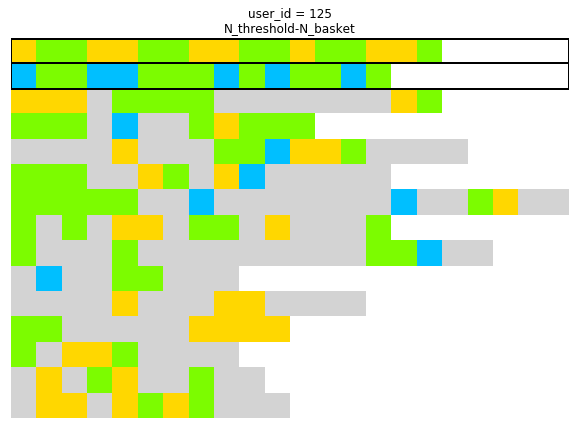
\includegraphics[height=\paperheight,width=\paperwidth]{../instacart-prediction-explorer/output_36_0.png}};
}

\begin{document}

\frame{

\titlepage}



\frame{\tableofcontents[hideallsubsections]}

\usebackgroundtemplate{%
}
\section{Introduction}
  \subsection%[Problem]
  {Problem: Predict the Items Instacart Costumers Purchase}
  \label{problem-predict-the-items-instacart-costumers-purchase}

\begin{frame}%{Problem: Predict the Items Instacart Costumers Purchase}

\begin{itemize}[<+->]
\item Instacart is a grocery-on-demand start-up which, in 2017, released a
dataset containing 3 million orders from 200,000 (anonymized) users. 
\vfill
\item A
now-completed Kaggle competition asked entrants to predict: Which
previously purchased products would be in a consumer's next order?
% In
%addition, Instacart would like to develop recommender systems that could
%predict which products a user would buy for the first time and which
%products would be added to a user's cart in future orders.
%
%Section \ref{top-n-variants} makes predictions according to the Kaggle
%competition, that is, from a given user's set of previously purchased
%products, predict which of those products the user will ultimately
%order. The 
\vfill
\item In addition to returning predictions to optimize traditional metrics, our
model includes product application variants for 

\begin{itemize}
  \item more precise predictions to, for example, populate a user's cart

  \item top-$N$ most-likely products a particular user will purchase to, for example, display on a web page of fixed results
\end{itemize}

\end{itemize}

\end{frame}



\subsection%[Data]
{Data: The Instacart Online Grocery Shopping Dataset}
\label{data-the-instacart-online-grocery-shopping-dataset}

\begin{frame}%{Data: The Instacart Online Grocery Shopping Dataset}

\begin{itemize}[<+->]
\item For each user, Instacart
provides between 4 and 100 of their orders, including the 
\begin{itemize}
\item intraorder sequence in which products were purchased, 
\item week and hour of the day the order was placed, 
\item relative time between orders, and
\item grocery store department to which each product belongs. 
\end{itemize}
\vfill

\item All data obtained from the Kaggle competition website. A relational 
set of \texttt{.csv} files which describe customer orders over
relative times. Each entity (customer, order, department, etc.) has a
unique id.
\vfill

\item A
\href{https://tech.instacart.com/3-million-instacart-orders-open-sourced-d40d29ead6f2}{blog
  post by Instacart} provides some information about the dataset and a
\href{https://www.kaggle.com/c/instacart-market-basket-analysis/overview}{Kaggle
  competition} provides additional details.


\end{itemize}

\end{frame}


  \subsection{Outline: Data Map Composition
}\label{outline-data-map-composition}


\begin{frame}%{Outline: Data Map Composition}
% The composition ? provides an overview
%Presentation structure corresponds to %the maps of 
%the composition 
\begin{block}{Structure}
\setlength\abovedisplayskip{0pt}
\begin{equation*}
\mathit{RawData}
\xmapsto{\quad \mathsf{P} \quad }
D 
\xmapsto{\quad \mathsf{F}\quad }
X
\xmapsto{\ \operatorname{\widehat{\mathsf{RFC}}}_\mathbf{n_0} }
\hat{y}^\star
\xmapsto{\ \mathsf{TopN}\ }
\hat{y}
\end{equation*}
\end{block}
\vfill
%as well as the domain and image.
\begin{description}[<+->]
\item[\(\mathit{RawData}\):] Exploratory Data Analysis
\item[\(\mathsf{P}\):] Partition \(\mathit{RawData}\) into $D_\text{train}$, $D_\text{test}$, \ldots
\item[\(\mathsf{F}\):] Feature Design builds design matrix $X$ from $D$
\item[\(\operatorname{\widehat{\mathsf{RFC}}}_\mathbf{n_0} \):] Random Forest Classifier makes probabilistic predictions \(\hat{y}^\star\) from $X$
\begin{itemize}
\item[\(\mathbf{n_0}\):] Hyperparameters found using \(\mathsf{OOB}\) classifier
\end{itemize}
\item[\(\mathsf{TopN}\):] TopN Variants make binary predictions \(\hat{y}\) from \(\hat{y}^\star\)
\item[\(\hat{y}\):] Prediction Explorer inspects binary predictions \(\hat{y}\)
\end{description}



%In section \ref{exploration} we perform exploratory data analysis on $\mathrm{RawData}$,
%the dataset described in section \ref{data-the-instacart-online-grocery-shopping-dataset}.
%Section \ref{train-test-split} describes the train/test partition $\mathsf{P}$.
%The feature design map $\mathsf{F}$ of section \ref{feature-design}
%assembles the partitioned raw data $D$ into a design matrix $X$
%which has user-product pairs as its rows. The random forest classifier
%$\mathsf{RFC}_{\mathbf{n_0}}$ of section \ref{random-forest-classifier}
%makes a probabilistic prediction $\hat{y}^\star$ of
%user-product pairs appearing in the user's ultimate order.
%In particular, section \ref{hyperparameter-tuning} locates optimal hyperparameters
%$\mathbf{n_0}$ for the random forest classifier.
%We devise various $\mathsf{TopN}$ schemes in section \ref{top-n-variants}
%to assign binary predictions $\hat{y}$.
%Finally, we exhibit a data visualization utility in section \ref{prediction-explorer} 
%to compare the predictions $\hat{y}$ against the true values $y_\text{test}$.


\end{frame}


\section%[RawData]
{Exploration}\label{exploration}

\subsection{RawData}

\begin{frame}%{\(\mathit{RawData}\): Exploratory Data Analysis}


\begin{table}[h]
  \centering
  \caption{\texttt{order\_products*.csv}}
  \label{tab:order-products}
  {\ttfamily
  \begin{tabular}{rrrr}
    \toprule
    order\_id & product\_id & add\_to\_cart\_order & reordered \\
    \midrule
    1         & 49302       & 1                    & 1         \\
    1         & 11109       & 2                    & 1         \\
    1         & 10246       & 3                    & 0         \\
    1         & 49683       & 4                    & 0         \\
    1         & 43633       & 5                    & 1         \\
    \bottomrule
  \end{tabular}
  }
%  \captionsetup{width=0.6\linewidth}
%  \caption*{While only \texttt{order\_products\_\_train.csv} is displayed, \texttt{order\_products\_\_prior.csv} has the same structure.}
\end{table}

Dictionaries \texttt{products.csv}, \texttt{aisles.csv}, and \texttt{departments.csv} provide a map from
\texttt{product\_id} to \texttt{product\_name}, \texttt{aisle\_id}, \texttt{aisle\_name}, \texttt{department\_id}, and \texttt{department\_name}.

\end{frame}

\begin{frame}
\begin{table}[h]
  \centering
  \caption{\texttt{orders.csv}}
  \label{tab:orders}
{\ttfamily
  \begin{tabular}{rrrrrrr}
    \toprule
    order\_id & user\_id & order\_num & dow & hour & days \\
    \midrule
    2539329   & 1             & 1             & 2          & 8                 & NaN               \\
    2398795   & 1             & 2             & 3          & 7                 & 15.0              \\
    473747    & 1             & 3             & 3          & 12                & 21.0              \\
    2254736   & 1            & 4             & 4          & 7                 & 29.0              \\
    431534    & 1             & 5             & 4          & 15                & 28.0              \\
    \bottomrule
  \end{tabular}
  }
\end{table}
\texttt{order\_num, dow, hour, \textsf{and} days} are abbreviations of \texttt{order\_number}, \texttt{order\_dow}, \texttt{order\_hour\_of\_day}, and \texttt{days\_since\_prior\_order}.


\end{frame}

\subsection{Temporal}


\begin{frame}
\begin{figure}[p]
    \begin{center}
    \adjustimage{max size={0.7\linewidth}{0.7\paperheight}}{../instacart-exploratory-data-analysis/output_64_0.png}
    \end{center}
    \caption[Heatmap of order times]{Saturday afternoon and Sunday morning are the most popular time to make
orders.}
     \label{fig:dow-vs-hr-order-heatmap}
\end{figure}

\end{frame}



\begin{frame}
 \begin{figure}[p]
\begin{center}
    \adjustimage{max size={0.9\linewidth}{0.9\paperheight}}{../instacart-exploratory-data-analysis/output_66_0.png}
\caption[Histogram of order frequency]{The most popular relative time between orders is monthly (30
days), but there are ``local maxima'' at weekly (7 days), biweekly (14
days), triweekly (21 days), and quadriweekly (28 days).}
\label{fig:days-histogram}
\end{center}
\end{figure}
\end{frame}


%----- Baskets Counts

\subsection{Baskets}

\begin{frame}
\begin{figure}[p]
\begin{center}
    \adjustimage{max size={0.9\linewidth}{0.9\paperheight}}{../instacart-exploratory-data-analysis/output_70_0.png}
\caption[Histogram of order counts by user]{Users have between 4 -- 100 orders. Those users in the dataset with 100 orders seem to have at least 100 orders and we have only their most recent 100 orders.}
\label{fig:orders-histogram}
\end{center}
\end{figure}
 
\end{frame}

\begin{frame}
\begin{figure}[p]
\begin{center}
    \adjustimage{max size={0.9\linewidth}{0.9\paperheight}}{../instacart-exploratory-data-analysis/output_73_0.png}
\end{center}
\caption[Histogram of basket sizes]{As one should expect, this distribution is right-skew. The mode basket size is 5.}
\label{fig:basket-size-histogram}
\end{figure} 
\end{frame}


\subsection{Product Popularity}


\begin{frame}
 \begin{table}%[t]{\textwidth}
\begin{tabular}{l>{\ttfamily}r}
\toprule
\texttt{product\_name}   & \texttt{count}        \\
\midrule
Banana                     & 491291 \\
Bag of Organic Bananas     & 394930 \\
Organic Strawberries       & 275577 \\
Organic Baby Spinach       & 251705 \\
Organic Hass Avocado       & 220877 \\
Organic Avocado            & 184224 \\
Large Lemon                & 160792 \\
Strawberries               & 149445 \\
Limes                      & 146660 \\
Organic Whole Milk         & 142813 \\
%Organic Raspberries        & 142603 \\
%Organic Yellow Onion       & 117716 \\
%Organic Garlic             & 113936 \\
%Organic Zucchini           & 109412 \\
%Organic Blueberries        & 105026 \\
%Cucumber Kirby             & 99728  \\
%Organic Fuji Apple         & 92889  \\
%Organic Lemon              & 91251  \\
%Organic Grape Tomatoes     & 88078  \\
%Apple Honeycrisp Organic   & 87272  \\
%Seedless Red Grapes        & 86748  \\
%Organic Cucumber           & 85005  \\
%Honeycrisp Apple           & 83320  \\
%Organic Baby Carrots       & 80493  \\
%Sparkling Water Grapefruit & 79245  \\ 
\bottomrule
\end{tabular}
%\captionsetup{width=.45\linewidth}
\caption{The most popular products are organic fruits or vegetables.}
\label{tab:top-products}
\end{table}
\end{frame}



\begin{frame}
%\caption[Reorder rates for products and aisles]{Reorder rates for products and aisles. 59.01\% of purchases were reorders.}
\begin{table}%[]{.5\textwidth}
\begin{tabular}{l>{\ttfamily}r}
\toprule
\texttt{product\_name}                                     & reorder \\
\midrule
Raw Veggie Wrappers                               & 0.9420       \\
Serenity Ultimate Extrema \ldots          & 0.9333       \\
%Serenity Ultimate Extrema Overnight Pads          & 0.9333       \\
Chocolate Love Bar                                & 0.9215       \\
Bars Peanut Butter                                & 0.8985       \\
Soy Crisps Lightly Salted                         & 0.8955       \\
Maca Buttercups                                   & 0.8942       \\
Benchbreak Chardonnay                             & 0.8918       \\
Organic Blueberry B Mega                          & 0.8888       \\
Sparking Water                                    & 0.8870       \\
Fragrance Free Clay \ldots & 0.8702       \\ 
%Fragrance Free Clay with Natural Odor Eliminat... & 0.8702       \\ 
\bottomrule
\end{tabular}
\caption{The most reordered products with at least 50 orders.}
\end{table}%
\end{frame}




\begin{frame}
\begin{table}%[]{.5\textwidth}
\begin{tabular}{ll>{\ttfamily}l}
\toprule
\texttt{aisle}                         & \texttt{department}    & \texttt{reorder} \\ 
\midrule
milk                          & dairy eggs    & 0.7818  \\
water seltzer\ldots & beverages     & 0.7299   \\
%water seltzer sparkling water & beverages     & 0.7299   \\
fresh fruits                  & produce       & 0.7188  \\
eggs                          & dairy eggs    & 0.7063  \\
soy lactosefree               & dairy eggs    & 0.6923  \\
...                           & ...           & ...       \\
beauty                        & personal care & 0.2128  \\
first aid                     & personal care & 0.1958  \\
kitchen supplies              & household     & 0.1948  \\
baking supplies \ldots         & pantry        & 0.1675  \\
spices seasonings             & pantry        & 0.1529  \\ 
\bottomrule
\end{tabular}
\caption{The most and least reordered from aisles.}
\end{table}
\label{tab:reorder-rates}
\end{frame}



\section{Partition}\label{partition}

\subsection{Partition Map}\label{partition-map}

\begin{frame}
\begin{columns}
\column{0.65\linewidth}
%The \emph{partition map} is a transformation,
\begin{block}{Partition RawData}
\setlength\abovedisplayskip{0pt}
\begin{equation*}\label{eq:partition-map}
\begin{split}
%   \mathsf{P} :
     \mathsf{RawData} &\xrightarrow{P} \mathsf{D}^{\textrm{DSets}} \\
     \mathrm{RawData} &\mapsto \{D_s\}_{s \in \textrm{DSets}}%,
\end{split}
\end{equation*}% 
\end{block}
%where
\column{0.35\linewidth}
\begin{block}{}
\centering
 \begin{tabular}{lr}
    \toprule
    eval\_set &  user\_id \\
    \midrule
%    prior    &   206209 \\
    train    &   131209 \\
    test     &    75000 \\
    \bottomrule
\end{tabular}
\end{block}
\end{columns}



% where
\begin{itemize}[<+->]
\item \(\mathrm{DSets} = \{\mathrm{train, test, kaggle}\}\),
\vfill
%\item \(\mathrm{RawData}\) denotes the collection of tables of user orders and
%baskets in \texttt{orders.csv} and \texttt{order\_products*.csv}, 
%\item \(\mathsf{RawData}\) is the set of possible collections of tables matching the column
%and relational structure of \(\mathrm{RawData}\),
\item \( \mathsf{P} \) is the unique partition defined by a partition of the set of users,
$U$, ordered by, say, \texttt{user\_id}, into $\{ U_s \}_{s \in \mathrm{DSets}}$% where the
%\href{https://scikit-learn.org/stable/modules/generated/sklearn.model_selection.train_test_split.html}{sklearn.model\_selection.train\_test\_split}
%utility determines the partition between \(U_\text{train}\) and
%\(U_\text{test}\), while \(U_\text{kaggle}\) consists of users whose \texttt{user\_id} is
%in a row matching the condition
%\texttt{ eval\_set == \textquotesingle{}test\textquotesingle{}} as follows
\vfill
\begin{itemize}
\item[\(U_\text{train}\):] 80\%
% of the 131,209 users whose ultimate orders are available.
of 131,209 users with available ultimate orders.
\vfill
\item[\(U_\text{test}\):] 20\% 
%of the 131,209 users whose ultimate orders are available. 
of 131,209 users with available ultimate orders.
\vfill
\item[\(U_\text{kaggle}\):] %The
75,000 users whose ultimate orders
are withheld by Kaggle.
% This project does not explicitly use this set;
%predictions on kaggle merely serve as a sanity check via submission to
%Kaggle.
\vfill
\end{itemize}
\item \(\{D_s\}_{s \in \mathrm{DSets}}\) is the image of $\mathrm{RawData}$ under $\mathsf{P}$.
%\item \(\ \mathsf{D}^{\mathrm{DSets}} \) are possible sets of the form \(\{D_s\}_{s \in \mathrm{DSets}}\),
%that is, the collection of possible partitions of members of \(\mathsf{RawData}\) over \( \mathrm{DSets} \).
\vfill
\end{itemize}

\end{frame}



\section{Feature Design}\label{feature-design}

\subsection{Feature Design Map}


\begin{frame}
 
\begin{block}{Feature Design}
\begin{equation*}\label{eq:feature-design}
\setlength\abovedisplayskip{0pt}
\begin{split}
  \mathsf{F}  :  \ \mathsf{D} &\rightarrow \mathsf{M}_{n\times m} (\mathbb{R}) \\
         D &\mapsto X
\end{split}
\end{equation*}
\end{block}
\vfill
\begin{itemize}
 \item \(\mathsf{F} = (\mathsf{f}_j )_{1}^m\) is an \(m\)-tuple of functions
%\begin{equation}
 \( \mathsf{f}_j : \mathsf{D} \rightarrow \mathbb{R}^n \)
%\end{equation} 
%calculates the \(j^\text{th}\) column of \(X\)
\vfill
\begin{itemize}
%%where
\item a \emph{feature} \( \mathsf{f}_j (D) \) is a %the \(j^\text{th}\) 
column of \(X\)
\vfill
\item \(\mathsf{f}_j\) are compositions of aggregations,
filtrations, arithmetic \ldots
\vfill
\item compute some \(\mathsf{f}_j\) via an
unsupervised learning technique,
\href{https://en.wikipedia.org/wiki/Latent_Dirichlet_allocation}{Latent
Dirichlet Allocation (LDA)}, introduced in
\cite{bleiLatentDirichletAllocation2003}.
\end{itemize}
\vfill
\item \(\mathop{Prod} (u)\) are all products purchased by \(u \in U\)
\vfill
\item Rows of \(X\) are user-product pairs
\begin{equation*}
\left( (u, p) \ | \ u \in U \ \& \ p \in \mathop{{Prod}} (u) \right)
\end{equation*}
\end{itemize}

\end{frame}


\subsection{Feature Source and Target}

\begin{frame}
 
\begin{itemize}
\item \(X \in \mathsf{M}_{n\times m} (\mathbb{R}) \) with shape values

\begin{table}
 \begin{tabular}{llll}
%\begin{longtable}[]{@{}llll@{}}
  \toprule
  \(n_\text{train}\) & \(n_\text{test}\) & \(n_\text{kaggle}\) &
  \(m\) \\
  \midrule
  \texttt{6760791}            & \texttt{1713870}           & \texttt{4833292}             & \texttt{47} \\
  \bottomrule
\end{tabular}
\end{table}
\vfill

\item Encode labels $y_\text{true} \in \{0,1\}^n$ as
\begin{equation*}
  y_\text{true}^{(u,p)} =
  \begin{cases}
    1  & \text{$u$ purchased $p$ in ultimate order}        \\
    0 & \text{$u$ did not purchase $p$ in ultimate order}
  \end{cases}
\end{equation*}
\vfill

\item Inspired by \cite{liuRepeatBuyerPrediction2016}, group features into a few Profiles:
\vfill
%\begin{longtable}[]{@{}ll@{}}
\begin{tabular}{ll}
%\caption[]{Profiles}\label{tbl:profiles} \\
  \toprule
%  prefix       & name\tabularnewline
%  \midrule
%  \endhead
  \texttt{U}   & User Profile\tabularnewline
  \texttt{P}   & Product Profile\tabularnewline
  \texttt{UP}  & User-Product Profile\tabularnewline
%  \texttt{AD}  & Aisle and Department Profiles (ignored)\tabularnewline
  \texttt{LDA} & Latent Dirichlet Allocation User Features\tabularnewline
  \bottomrule
\end{tabular}
%\end{longtable}


\end{itemize}
 
 
 
\end{frame}




\subsection{Feature Examples}

\begin{frame}

\begin{center}
\begin{tabular}{>{\ttfamily}l>{\ttfamily}lp{4cm}} \toprule
  \textsf{feature}                                  & \textsf{dtype}                                     & description  \\ \midrule
   U\_items\_total                        &                        uint16           & number of total items a given user has purchased\\ \hline
    U\_reordered\_ratio                    &                    float16              & proportion of items a given user has purchased which are reorders\\ \hline
       P\_unique\_users                       &                       uint16            & number of purchasers\\ \hline
    UP\_order\_ratio                       &                       float16           & fraction of baskets in which a given product appears for a given user (count of orders in which product appears divided by total orders) \\ \hline
    UP\_penultimate                        &                       bool              & product in user's penultimate (previous) order\\                                                                                                                                                                                                                                                                                                                
   \bottomrule
\end{tabular}
\end{center}

\end{frame}



\section%[RFC]
{Random Forest Classifier}

\subsection{Random Forest Classifier Map; Review}

\begin{frame}
\begin{block}{Random Forest Classifier Map}
\begin{equation*}\label{eq:RFC-Theta}
\begin{gathered}
\operatorname{\widehat{\mathsf{RFC}}}_\mathbf{n_0} : 
\mathsf{M}_{n \times m} (\mathbb{R}) \rightarrow [0, 1]^n \\ 
X \mapsto \hat{y}^\star
\end{gathered}
\end{equation*}
for a(n optimal) choice of hyperparameters $\mathbf{n_0}$; number of trees $B$.
\end{block}
\vfill
\begin{itemize}
 \item \Summertree s: information criterion determines recursive binary 
 splittings by hyperplanes $\perp$ axes
 \vfill
 \item \Summertree classifier: $\mathbf{n}$ determines distribution on \Summertree topology; \\
 empirical risk minimization with respect to some loss $L$
 \vfill
 \item \(\operatorname{\widehat{\mathsf{RFC}}}_\mathbf{n}\):  average \Summertree estimators on bootstrap samples $(\mathbf{Z}^*_b)_{b \leq B}$ but limit dimensions considered in splittings to \texttt{max\_features}
 \vfill 
\item$\hat{y}^\star$ is \emph{probabilistic prediction} --  interpret as probability ranking
\end{itemize}

 \end{frame}

\subsection{Out-Of-Bag (OOB) Classifier}
%\subsection[\(\mathbf{n}_0\)]{Hyperparameter Search}

\begin{frame}
 
\begin{itemize}
 \item $\mathbf{Z}^*_b$ only includes 2/3 of samples -- 
 use the remaining 1/3 to obtain the corresponding out-of-bag (OOB) classifier
 \begin{equation*}
 \operatorname{\widehat{\mathsf{OOB}}}_\mathbf{n} : \mathsf{M}_{n \times m} (\mathbb{R})  \rightarrow [0, 1]^n
\end{equation*}
 \vfill
 \item OOB error $\gtrapprox$ test error
  \vfill
 \item Use OOB error \alert{(on train!)} instead of $N$-fold cross-validation
 \begin{itemize}
 \item Simplifies phases of project
 \item $N$-fold cross-validation is memory-intensive in splitcopy data
 \end{itemize}
   \vfill
 \item OOB rank metric scores for $\{  \operatorname{\widehat{\mathsf{OOB}}}_\mathbf{n} \}_{\mathbf{n} \in \mathbf{G}}$,
$\mathbf{G}$ a \emph{parameter grid},
 \begin{itemize}
 \item $\mathtt{min\_samples\_leaf} \in \{12, 24, 48\}$,
\item $\mathtt{min\_impurity\_decrease} \in [10^{-8}, 10^{-7.5}, 10^{-7}, 10^{-6.5}, 10^{-6}]$,
\item[$+$] \texttt{sklearn.ensemble.RandomForestClassifier} defaults
\end{itemize}
 \end{itemize}

\end{frame}

\subsection{\(\mathbf{n}_0\): Hyperparameters Optimize OOB Error}

\begin{frame}
 \begin{figure}[p]
\begin{center}
    \adjustimage{max size={0.9\linewidth}{0.9\paperheight}}{../instacart-random-forest-parametergrid-search/output_31_0_crop.png}

\end{center}
\end{figure}
\begin{itemize}
\item AUC-PR may be more relevant than AUC-ROC since
\begin{equation*}
\text{skew} = \frac{\text{Negative Classes}}{\text{Positive Classes}} \approx 10 
\end{equation*}
\item AUC-PR argmax occurs close to AUC-ROC argmax: 
$\mathbf{n_0} = (\mathtt{min\_impurity\_decrease = 10^{-6.5}},$\\
  $\mathtt{min\_samples\_leaf = 24},
 \ldots )$

\end{itemize}
\end{frame}


\subsection{Receiver Operating Characteristic (ROC) curve}

\begin{frame}
 \begin{figure}[p]
\centering
    \adjustimage{max size={0.7\linewidth}{0.7\paperheight}}{../instacart-top-n-random-forest-model/output_17_0.png}
\caption[ROC Curve]{Receiver Operating Characteristic (ROC) curve for 
$\operatorname{\widehat{\mathsf{RFC}}}_\mathbf{n_0}$; AUC-ROC = 0.83.}
\label{fig:roc}
\end{figure}
\end{frame}

\subsection{Precision-Recall Curve}

\begin{frame}
\begin{figure}[p]
\centering
    \adjustimage{max size={0.7\linewidth}{0.7\paperheight}}{../instacart-top-n-random-forest-model/output_19_0.png}
\caption[Precision-Recall Curve]{Precision-Recall Curve for 
$\operatorname{\widehat{\mathsf{RFC}}}_\mathbf{n_0}$; AUC-PR = 0.41.}
\label{fig:precision-recall}
\end{figure}
\end{frame}

\subsection{Variable Importances}

\begin{frame}
 \begin{figure}[]
\centering
    \adjincludegraphics[height=0.6\paperheight, width=0.8\paperwidth, trim={0 300 0 0},clip]{../instacart-top-n-random-forest-model/output_11_0.png}
\caption[\texttt{RandomForestClassifier} Variable Importance]{The \texttt{RandomForestClassifier} uses an information criterion to determine variable importances. There's still gold to mine in {\color{gold} \texttt{UP}} !}
\label{fig:variable-importances}
\end{figure}
\end{frame}



\section{TopN}

\subsection{TopN Map; Variants}

\begin{frame}
 
 \begin{block}{TopN Variants}
\setlength\abovedisplayskip{0pt}
\begin{equation*}\label{eq:top-n}
\begin{split}
\operatorname{\mathsf{TopN}} : {[0, 1]}^{n} &\rightarrow \{0, 1\}^n \\ 
\hat{y}^\star  &\mapsto \hat{y}
\end{split}
\end{equation*}% 
\end{block}
 
\begin{itemize}
 \item $\operatorname{\mathsf{TopN}}$ maps make binary predictions from probability rankings
\begin{description}
 \item[$\operatorname{\mathsf{TopN}}_\text{threshold}$] chooses a classification threshold $p_0$;\\
 best for optimizing threshold metrics (F1-score); not best for product applications
\item[$\operatorname{\mathsf{TopN}}_\text{u}$] uses user's mean basket size as $N$;\\
set basket size by user reduces its variance;
higher precision versions to autopopulate carts?
\item[$\operatorname{\mathsf{TopN}}_\text{N}$]  uses a constant value $N$ for each user;\\
worse metrics but best for displaying on fixed-width web page (zero basket size variance)
\end{description}
\end{itemize}
\end{frame}


\subsection{$\operatorname{\mathsf{TopN}}_\text{threshold}$}

\begin{frame}
 \begin{figure}[]
\centering
   \adjustimage{max size={0.9\linewidth}{0.9\paperheight}}{../instacart-top-n-random-forest-model/output_38_0.png}
\caption{Scores for \(\mathsf{TopN\_\textsf{threshold}}\) variants.}
\label{fig:n-threshold-scores}
\end{figure}
\end{frame}

\begin{frame}
 \begin{figure}[]
\begin{center}
   \adjustimage{max size={0.75\linewidth}{0.75\paperheight}}{../instacart-top-n-random-forest-model/output_47_0.png}
\caption{Normalized confusion matrices for \(\mathsf{TopN\_\textsf{threshold}}\) variants.}
\label{fig:n-threshold-confusion}
\end{center}
\end{figure}
\end{frame}


\subsection{$\operatorname{\mathsf{TopN}}_\text{u}$}



\begin{frame}
 
\begin{figure}[t]
\begin{center}
   \adjustimage{max size={0.9\linewidth}{0.9\paperheight}}{../instacart-top-n-random-forest-model/output_58_0.png}
\caption{Scores for $\mathsf{TopN_u}$ variants.}
\label{fig:n-u-scores}
\end{center}
\end{figure}
\end{frame}

\begin{frame}
\begin{figure}[h!]
\begin{center}
   \adjustimage{max size={0.9\linewidth}{0.9\paperheight}}{../instacart-top-n-random-forest-model/output_61_0.png}
\caption{Normalized confusion matrices for $\mathsf{TopN_u}$ variants.}
\label{fig:n-u-confusion}
\end{center}
\end{figure}
\end{frame}



\subsection{$\operatorname{\mathsf{TopN}}_\text{N}$}


\begin{frame}
 

\begin{figure}[t!]
\begin{center}
   \adjustimage{max size={\linewidth}{0.75\paperheight}}{../instacart-top-n-random-forest-model/output_67_0.png}
\caption{Scores for $\mathsf{TopN_N}$ variants.}
\label{fig:top-n-scores}
\end{center}
\end{figure}
\end{frame}

\begin{frame}
 

\begin{figure}[]
\begin{center}
   \adjustimage{max size={0.9\linewidth}{0.9\paperheight}}{../instacart-top-n-random-forest-model/output_70_0.png}
\caption{Normalized confusion matrices for $\mathsf{TopN_N}$.}
\label{fig:top-n-confusion}
\end{center}
\end{figure}
\end{frame}

\section{Prediction Explorer}

\subsection{Color Palette}

\begin{frame}{Prediction Explorer}
 
Given a user and a model variant, visualize the model prediction, true order, and basket history,
with colorings for
\vfill
\begin{itemize}
\item \(\color{lawngreen}{\text{True Positives: Ordered and Predicted}}\) \vfill
\item \(\color{gold}{\text{False Positives: Predicted but not Ordered}}\) \vfill
\item \(\color{deepskyblue}{\text{False Negatives: Ordered but not Predicted}}\) \vfill
\item \(\color{lightgrey}{\text{True Negatives: neither Ordered nor Predicted}}\) \vfill
\end{itemize}
\vfill
A model with greater \textbf{precision} has fewer
\(\color{gold}{\text{False Positives}}\);\\% while
A model with greater
\textbf{recall} has fewer
\(\color{deepskyblue}{\text{False Negatives}}\).\\
Note: \texttt{\textquotesingle{}add\_to\_cart\_order\textquotesingle{}}
is not meaningful for the top rows of predictions and true orders.

\end{frame}

\subsection{Styled DataFrame Excerpt}

\begin{frame}
\begin{figure}[]
\begin{center}
   \adjustimage{max size={0.9\linewidth}{0.75\paperheight}}{../instacart-prediction-explorer/styled_df.png}
\caption[
%Styled DataFrame of Predictions, Ultimate Orders, and Basket History
]{
%A portion of a styled DataFrame of Predictions, Ultimate Orders, and Basket History for
%\texttt{
%user\_id == \PY{n}{users}\PY{p}{[}\PY{l+s+s1}{\PYZsq{}}\PY{l+s+s1}{test}\PY{l+s+s1}{\PYZsq{}}\PY{p}{]}\PY{p}{[}\PY{l+m+mi}{18}\PY{p}{]}
%};
\texttt{user\_id == 125};
\texttt{
model ==  
(\textquotesingle{}N\_threshold\textquotesingle{},
\textquotesingle{}N\_basket\textquotesingle{})
% \PY{p}{(}\PY{l+s+s1}{\PYZsq{}}\PY{l+s+s1}{N\PYZus{}threshold}\PY{l+s+s1}{\PYZsq{}}\PY{p}{,} \PY{l+s+s1}{\PYZsq{}}\PY{l+s+s1}{N\PYZus{}basket}\PY{l+s+s1}{\PYZsq{}}\PY{p}{)}\PY{p}
}
}
\label{fig:styled-df}
\end{center}
\end{figure}
\end{frame}

\subsection{Confusion Basket History}

\begin{frame}
 \begin{figure}[]
%\caption[Style of Predictions, Ultimate Orders, and Basket History]{``Zoom out'' on Figure \ref{fig:styled-df} by ignoring product names.}
\begin{center}
    \adjustimage{max size={0.9\linewidth}{0.9\paperheight}}{../instacart-prediction-explorer/output_36_0.png}
\end{center}
\caption{``Zoom out'' by ignoring product names.}
\label{fig:style}
\end{figure}

\end{frame}



\begin{frame}
 
\begin{figure}
\begin{center}
    \adjustimage{max size={\linewidth}{0.9\paperheight}}{../instacart-prediction-explorer/output_38_0.png}
\caption[%Model Variant Prediction Exploration for a Fixed User
]
{``Zoom out'' further by displaying predictions for \texttt{user\_id == 125} using a few model choices. By fixing a user, we can inspect the behavior of different models.}
\label{fig:models-styles}
\end{center}
\end{figure}

\end{frame}


\begin{frame}

\begin{figure}[]
\begin{center}
    \adjincludegraphics[height=0.75\paperheight, width=0.70\paperwidth, trim={0 676 0 0},clip]{../instacart-prediction-explorer/output_39_0.png}
\caption[Prediction Exploration for Varying User and Model]{Zoom out on Figure \ref{fig:models-styles} to include more users.}
\label{fig:users-models-styles}
\end{center}
\end{figure}

\end{frame}

\begin{frame}

\begin{figure}[]
\begin{center}
    \adjincludegraphics[height=0.75\paperheight, width=0.70\paperwidth, trim={0  0 0 676},clip]{../instacart-prediction-explorer/output_39_0.png}
\caption[Prediction Exploration for Varying User and Model]{Zoom out on Figure \ref{fig:models-styles} to include more users.}
\label{fig:users-models-styles}
\end{center}
\end{figure}

\end{frame}



\section{References}

\nocite{hastieElementsStatisticalLearning2009}
%\nocite{breimanRandomForests2001}
\bibliographystyle{alpha}
\bibliography{instacart-presentation}{}



%  \begin{itemize}
%  \item<1-> Normal LaTeX class.
%  \item<2-> Easy overlays.
%  \item<3-> No external programs needed.      
%  \end{itemize}



\end{document}
